\documentclass[]{article}

\usepackage{tabularx}
\usepackage[dutch]{babel}
\usepackage{amsmath}
\usepackage{graphicx}
\usepackage{amsmath}
\usepackage{epstopdf}
\usepackage[parfill]{parskip}

\newcommand{\opgave}[1]{\section*{Opgave #1}}

\begin{document}

\opgave5

\begin{figure}
\noindent 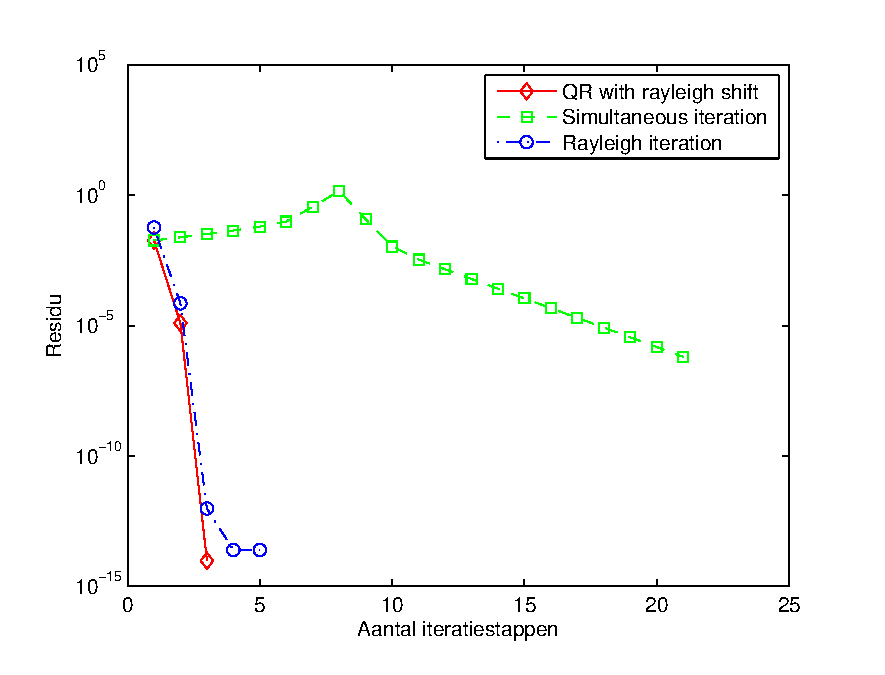
\includegraphics[width=1\linewidth]{Opgave5.eps}
\caption{Convergentie}
\label{figuurtje}
\end{figure}



Aangezien we hier de gelijktijdige iteratie uitvoeren met I als de start matrix is deze methode hetzelfde als de QR methode zonder shifts. Deze convergeert dus linear net zoals de methode van de machten. De QR methode met rayleigh quotient shift convergeert cubisch. Deze methode is eigenlijk dezelfde methode als de rayleigh iteratie, maar dan in Matrix vorm. Alhoewel het dus veel meer rekenwerk vraagt per iteratie voor de QR methode met rayleigh  shift om alle eigenwaarden te berekenen dan de de rayleigh iteratie om 1 eigenwaarde te berekenen convergeren de methodes in ongeveer evenveel iteraties naar correcte eigenwaarden.
\end{document}